\oldpage{399}\begin{figure}[H]
  \centering
  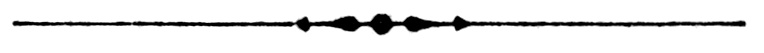
\includegraphics{pages/illustrations/arrow_bullet_divider.jpg}
\end{figure}
\section*{Extractum Nicotianiæ Rademacheri.}

\byline*{\ProperName{Theodore~C.\ Miller},\ \md}

\SectionStartWords{I herewith} present a notice of an agent which to me is possessed of
extreme value. It is the \emph{extract of the Nicotiania rustica}, as prepared
by the late Dr.\ T.~G.\ Rademacher.

It is not prepared from the dry but from the fresh and green tobacco
plant. In preparing the extract it is necessary that \emph{immediately} and
without delay, after the leaves have been pulled they must be pressed
so as to force out the juice and that juice evaporated to the consistency
of an extract. When prepared in this manner the extract has none of
the taste of the dried tobacco leaves; but if the leaves are pulled only
a few hours before the juice is expressed, then the extract will have a
taste more or less like that of smoking tobacco, in which case it is not
fit for therapeutical purposes. I have ahvays found it best to have the
leaves pressed at once on being pulled; and I have always prepared it
according to the directions of Rademacher, from the Nicotiania rustica,
and not from the Nicotiania tabacum. Rademacher's extract is one of
the best remedies in genuine cough of the lungs, and for that I can wdth
a clear conscience recommend it to the readers of the \ThisJournal{College Journal}.
It is a remedy for which probably I could not find a substitute.

Rademacher gave it in doses of from one half to two grains, and repeated
it several times a day. It may be made into a pill with the
powdered marsh mallow root. It is a quick and safe remedy in a particular
diseased condition of the lungs for which I am not able to give
a name, but the want of the \emph{name} is no loss to the practical physician,
who must be governed by the nature of the disease and not by its
nomenclature.

That we can, with the extract of the fresh leaves of tobacco, cure an
inveterate genuine lung cough, and thus prevent pulmonary tuberculosis,
in my mind does not admit of a doubt, provided the cough is kept under
the control of the remedy. But there are forms of lung cough which
this extract will not control, and in those cases I would recommend a
trial of the \emph{Stibium Sulphuretum Auranticum}, as mentioned in the
\ThisJournal{College Journal} for June, page 351. Rademacher truly says: ``In
general we must be guided in our minds in the practice of our art, by
the following fact: The diseases are not governed or changed in character
by the ideas and opinions of the physician, but the opinion of
the physician must be governed by the nature of the disease.''

That the extract of tobacco has a powerful controlling influence over\endinput
